\documentclass[10pt, handout]{beamer}

\usetheme[progressbar=frametitle]{metropolis}

\usepackage{appendixnumberbeamer}

\usepackage{booktabs}
\usepackage{blkarray}
\usepackage{ccicons}
\usepackage{graphicx}
\usepackage{color}
\usepackage{subcaption}


\definecolor{UniBlue}{RGB}{7,82,154}
\definecolor{UniYellow}{RGB}{234,185,12}

%\setbeamercolor{title}{fg=UniBlue, bg = UniYellow}
%\setbeamercolor{frametitle}{fg=UniBlue, bg= UniYellow}
%\setbeamercolor{structure}{fg=UniBlue, bg= UniYellow}
%\setbeamercolor{progress bar}{fg=UniBlue, bg= UniYellow}
\usepackage{xspace}

\title{Estimation of the Long-run Error Variance in Nonparametric Regression with Time Series Errors}
\date{EcoSta 2023}
\author{Marina Khismatullina \inst{1} \and Michael Vogt \inst{2}}
<<<<<<< HEAD
\institute{\inst{1} Erasmus University Rotterdam \\ \inst{2} Ulm University}
=======
\institute{\inst{1} Erasmus University Rotterdam \\\inst{2} Ulm University}
>>>>>>> 20d15732727bc5ea2037f88bbcaf3c6629a43244
\setbeamertemplate{frame footer}{Estimation of the Long-run Error Variance}
\metroset{block=fill}
% \titlegraphic{\hfill\includegraphics[height=1.5cm]{logo.pdf}}

\newcommand{\Prob}{\mathrm{P}}
\newcommand{\E}{\mathbb{E}}
\newcommand{\Var}{\mathrm{Var}}
\newcommand{\Cov}{\mathrm{Cov}}
\newcommand{\Corr}{\mathrm{Corr}}
\newcommand{\sgn}{\text{sgn}}
\newtheorem{prop}{Proposition}


\begin{document}

\maketitle

%\begin{frame}{Table of contents}
%  \setbeamertemplate{section in toc}[sections numbered]
%  \tableofcontents[hideallsubsections]
%\end{frame}

\section{Introduction}



%\begin{frame}{Idea}
%    \begin{block}{Research question}
%	Develop multiscale methods to test qualitative hypotheses about nonapametric time trends.\pause
%	
%	One time series is observed:
%	\begin{itemize}
%		\item Test the null hypothesis of the existence of a time trend.
%		\item Identify time regions with upward or downward movement in the trend.
%	\end{itemize}\pause
%	Multiple time series are observed:
%	\begin{itemize}
%		\item  Detect which time trends are different and where.
%	\end{itemize}
%    \end{block}
%\end{frame}

\begin{frame}{Model}
We observe a single time series $\{Y_t: 1 \le t \le T \}$ of length $T$. The observations come from the following model:
\begin{equation*}\label{model1}
Y_t = m \Big( \frac{t}{T} \Big) + \varepsilon_t 
\end{equation*}
\vspace{-6mm}
\begin{itemize}
\item $m$ is an unknown trend function on $[0,1]$;
\item $\{ \varepsilon_t: 1 \le t \le T \}$ is a zero-mean stationary and causal error process.\pause
\end{itemize}\begin{block}{Problem}
Estimate the long-run error variance $\sigma^2 = \sum\nolimits_{\ell=-\infty}^{\infty} \Cov(\varepsilon_0,\varepsilon_{\ell})$.
\end{block}

\end{frame}

\begin{frame}{Literature}
	Residual-based approach: estimate $\sigma^2$ from the residuals $$\widehat{\varepsilon}_t = Y_t - \widehat{m}\left(\frac{t}{T}\right)$$
	\vskip -2mm
	\begin{itemize}
		\item AR($p$) error processes (Truong, 1991; Shao and Yang, 2011; Qiu et al., 2013)
	\end{itemize}\pause
	Difference-based approach: estimate $\sigma^2$ from the $\ell$-th differences $Y_t - Y_{t-\ell}$.
	\begin{itemize}
		\item AR($p$) error processes (Hall and Van Keilegom, 2003) 
		\item MA($m$) error processes (M{\"u}ller and Stadtm{\"u}ller, 1988; Herrmann et al., 1992; Tecuapetla-G{\'o}mez and Munk, 2017)
	\end{itemize}
\end{frame}



%\section{Theoretical properties}
%\begin{frame}{Assumptions}
%\begin{itemize}
%\onslide<1->\item[$\mathcal{C}1$] \label{C-err1} The variables $\varepsilon_t$ are weakly dependent.
%\onslide<2->\item[$\mathcal{C}2$] \label{C-err2} It holds that $\| \varepsilon_t \|_q < \infty$ for some $q > 4$.
%\onslide<3->\item[$\mathcal{C}3$] \label{C-ker} Standard assumptions on the kernel function $K$.
%\onslide<4->\item[$\mathcal{C}4$] Assume that  $\widehat{\sigma}^2 = \sigma^2 + o_p(\rho_T)$ with $\rho_T = o(1/\log T)$.
%\onslide<5->\item[$\mathcal{C}5$] \label{C-grid} $|\mathcal{G}_T| = O(T^\theta)$ for some arbitrarily large but fixed constant $\theta > 0$.
%\begin{overprint}
%\onslide<6>
%\vspace{-3mm}
%\begin{align*}
%\mathcal{G}_T = \big\{ & (u,h): u = t/T \text{ for some } 1 \le t \le T \text{ and } h \in [h_{\min},h_{\max}] \\ & \text{ with } h = t/T \text{ for some } 1 \le t \le T  \big\},
%\end{align*}
%\onslide<7>
%\vspace{-3mm}
%\item[$\mathcal{C}6$] \label{C-h} $h_{\min} \gg T^{-(1-\frac{2}{q})} \log T$ and $h_{\max} = o(1)$.
%
%\end{overprint}
%\end{itemize}
%\end{frame}
\section{Model}

\begin{frame}{Setting}
Estimate the long-run error variance $\sigma^2 = \sum\nolimits_{\ell=-\infty}^{\infty} \Cov(\varepsilon_0,\varepsilon_{\ell})$ of the error terms $\{\varepsilon_t\}$ in the model 
\begin{equation*}
Y_t = m \Big( \frac{t}{T} \Big) + \varepsilon_t, 
\end{equation*}
where $m(\cdot)$ is Lipshitz and $\{\varepsilon_t\}$ is an AR($p^\star$) process of the form 
\begin{equation*}
\varepsilon_t = \sum_{j=1}^{p^\star} a_j \varepsilon_{t-j} + \eta_t. 
\end{equation*} \pause
\vspace{-3mm}
\begin{itemize}
	\item $a_1, a_2, a_3,\ldots$ are the unknown parameters;\pause
	\item $\eta_t$ are i.i.d.\ innovations with $\E[\eta_t] = 0$ and $\E[\eta_t^2] = \nu^2$;\pause
	\item $p^\star \in \mathbb{N} \cup \{\infty\}$ is unknown.\pause Two possible cases: 
\begin{itemize}
	{\color<6>{mLightBrown}\item[(A)] $p^\star$ is not known but we know an upper bound $p$ on it;}
	\item[(B)] or we neither know $p^\star$ nor an upper bound on it. 
\end{itemize}
\end{itemize}\pause
\end{frame}


\begin{frame}{Setting}
We assume that 
\begin{equation*}
A(z) := 1 - \sum_{j=1}^{p^\star} a_j z^j \neq 0
\end{equation*}
for all complex numbers $|z|\leq 1+ \delta$ with some small $\delta >0$.\pause

Therefore,

\begin{itemize}
	\item the error process $\{\varepsilon_t\}$ is stationary and causal;\pause
	\item the coefficients $a_1, a_2, a_3,\ldots$ decay to zero exponentially fast;\pause
	\item $\{\varepsilon_t\}$ has an MA($\infty$) representation of the form $\varepsilon_t = \sum_{k=0}^\infty {\color<5>{mLightBrown}c_k} \eta_{t-k}$.
\end{itemize}
\end{frame}

\section{Estimation}

\begin{frame}{Motivation for the estimator}
If $\{\varepsilon_t\}$ is an AR($p^\star$) process, then the time series $\{ \Delta_q \varepsilon_t \}$ of the differences $\Delta_q \varepsilon_t = \varepsilon_t - \varepsilon_{t-q}$ is an ARMA($p^\star,q$) process of the form 
\begin{equation*}
\Delta_q \varepsilon_t - \sum_{j=1}^{p^\star} a_j \Delta_q \varepsilon_{t-j} = \eta_t - \eta_{t-q}. 
\end{equation*}\pause

Then, since the trend function $m(\cdot)$ is Lipshitz, $\Delta_q Y_{t} = Y_{t} - Y_{t-q}$ is approximately an ARMA($p^\star,q$) process.
\end{frame} 


\begin{frame}{Yule-Walker equations}
For any differencing order $q \geq 1$, we have
\vspace{-3mm}
\begin{align*}
	\gamma_q(\ell) - \sum_{j=1}^{p^\star} a_j \gamma_q(\ell - j) = \begin{cases}
	-\nu^2 c_{q - \ell} &\text{ for } 1\leq \ell < q+1,\\
	0 &\text{ for } \ell \geq q+1.
	\end{cases}
\end{align*}
where
\vspace{-3mm}
\begin{itemize}
	\item $\boldsymbol{c}_q = (c_{q-1},\dots,c_{q-p})^\top$ are the coefficients from the MA($\infty$) expansion of $\{ \varepsilon_t \}$;
	\item $\boldsymbol{\gamma}_q = (\gamma_q(1),\dots,\gamma_q(p))^\top$ with $\gamma_q(\ell) = \Cov(\Delta_q \varepsilon_t,$ $\Delta_q \varepsilon_{t-\ell})$;
	\item and $\boldsymbol{\Gamma}_q$ is the $p \times p$ covariance matrix $\boldsymbol{\Gamma}_q = (\gamma_q(i-j): 1 \le i,j \le p)$.
\end{itemize}\pause
\begin{block}{In vector notation}
\begin{equation*}\label{YU-eq}
\boldsymbol{\Gamma}_q \boldsymbol{a} = \boldsymbol{\gamma}_q + \nu^2{\color<3>{mLightBrown} \boldsymbol{c}_q}  -  {\color<3>{mLightBrown}\boldsymbol{\rho}_q}
\end{equation*}
\end{block}
\vspace{-2mm}
where $\boldsymbol{\rho}_q = (\rho_q(1), \ldots, \rho_q(p))$ with $\rho_q(\ell) = \sum_{j=p+1}^{p^\star} a_j \gamma_q(\ell - j)$.
\end{frame}

\begin{frame}{Estimator, first stage}

\begin{block}{Note}
\vspace{-3mm}
\begin{center}
$\boldsymbol{\Gamma}_q \boldsymbol{a} \approx \boldsymbol{\gamma}_q$ for large values of $q$.
\vspace{-3mm}
\end{center}\end{block}\pause

We construct the first-stage estimator by
\begin{equation*}
\widetilde{\boldsymbol{a}}_q = \widehat{\boldsymbol{\Gamma}}_q^{-1} \widehat{\boldsymbol{\gamma}}_q, 
\end{equation*}
where $\widehat{\boldsymbol{\Gamma}}_q$ and $\widehat{\boldsymbol{\gamma}}_q$ are constructed from the sample autocovariances $$\widehat{\gamma}_q(\ell) = (T-q)^{-1} \sum_{t=q+\ell+1}^T \Delta_q Y_{t} \Delta_q Y_{t-\ell}.$$ 
\end{frame}

\begin{frame}{Tuning parameter}
\begin{equation*}
\widetilde{\boldsymbol{a}}_q = \widehat{\boldsymbol{\Gamma}}_q^{-1} \widehat{\boldsymbol{\gamma}}_q 
\end{equation*}
\vspace{-3mm}
\begin{block}{Problem}
How to choose $q$?
\end{block}\pause
\vspace{-2mm}
\begin{itemize}
	\item[(i)] $q$ should be large enough so that $\boldsymbol{c}_q = (c_{q-1},\dots,c_{q-p})^\top$ is close to zero;\pause
	\item[(ii)] $q$ should not be too large to sufficiently eliminate the trend.
\end{itemize}\pause
In case of AR($1$), $q= 20$ is enough.\pause

For the consistency, we need $\log T \ll q \ll \sqrt{T}$.
\end{frame}

\begin{frame}{Estimator, second stage}
\begin{block}{Problem}
If the trend $m$ is pronounced, the estimator $\widetilde{\boldsymbol{a}}_q$ will have a strong bias.
\end{block}\pause
\vspace{-2mm}
Solution:
\begin{itemize}
	\item \vspace{-2mm} Compute estimators $\widetilde{c}_k$ of $c_k$ based on $\widetilde{\boldsymbol{a}}_q$.\pause
	\item Estimate the innovation variance $\nu^2$ by $\widetilde{\nu}^2 = (2T)^{-1} \sum_{t=p+2}^T \widetilde{r}_{t}^2$, where $\widetilde{r}_{t} = \Delta_1 Y_{t} - \sum_{j=1}^p \widetilde{a}_j \Delta_1 Y_{t-j}$.\pause
	\item Estimate $\boldsymbol{a}$ by 
\begin{equation*}\label{est-AR-SS} 
\widehat{\boldsymbol{a}}_r = \widehat{\boldsymbol{\Gamma}}_r^{-1} (\widehat{\boldsymbol{\gamma}}_r + \widetilde{\nu}^2 \widetilde{\boldsymbol{c}}_r).
\end{equation*}\pause
	\item \vspace{-4mm} Average the estimators $\widehat{\boldsymbol{a}}_r$: $\widehat{\boldsymbol{a}} = \frac{1}{\overline{r} - \underline{r} + 1} \sum\limits_{r=\underline{r}}^{\overline{r}} \widehat{\boldsymbol{a}}_r$.\pause
	\item Estimate the long-run variance $\sigma^2$ by 
\begin{equation*} \label{est-lrv}
\widehat{\sigma}^2 = \frac{\widehat{\nu}^2}{(1 - \sum_{j=1}^p \widehat{a}_j)^2}. 
\end{equation*}
\end{itemize}
\end{frame}



\begin{frame}{Tuning parameter}
\begin{equation*}\label{est-AR-SS} 
\widehat{\boldsymbol{a}}_r = \widehat{\boldsymbol{\Gamma}}_r^{-1} (\widehat{\boldsymbol{\gamma}}_r + \widetilde{\nu}^2 \widetilde{\boldsymbol{c}}_{\color<2-3>{mLightBrown}r})
\end{equation*}\pause
\vspace{-5mm}
\begin{itemize}
	\item[(i)] $r$ is a much smaller differencing order than $q$;\pause
	\item[(ii)] $r \geq 1$ is sufficient.
\end{itemize}\pause
$$\widehat{\boldsymbol{a}} = \frac{1}{\overline{r} - \underline{r} + 1} \sum\limits_{r=\underline{r}}^{\overline{r}} \widehat{\boldsymbol{a}}_r$$
\vspace{-3mm}

\begin{block}{Problem}
How to choose $\underline{r}$ and $\overline{r}$?
\end{block}\pause

We choose them to be fixed (small) natural numbers. Simulations in the paper.

\end{frame}


\begin{frame}{Theoretical properties}
Performance:
\begin{itemize}
\item Our estimator $\widehat{\boldsymbol{a}}$ produces accurate estimation results even when the AR polynomial $A(z) = 1 - \sum_{j=1}^{p^\star} a_j z^j$ has a root close to the unit circle.\pause
\item Our pilot estimator $\widetilde{\boldsymbol{a}}_q$ tends to have a substantial bias when the trend $m$ is pronounced. The second-stage estimator $\widehat{\boldsymbol{a}}$ reduces this bias considerably.\pause
\end{itemize}
\begin{prop}{}
Our estimators $\widetilde{\boldsymbol{a}}_q$, $\widehat{\boldsymbol{a}}$ and $\widehat{\sigma}^2$ are $\sqrt{T}$-consistent. 
\end{prop}
\end{frame}

\section{Simulations}

\begin{frame}{Simulations}
Setting:
\begin{itemize}
\item data from the model $Y_t = m(t/T) + \varepsilon_t$, where $\varepsilon_t$ is an AR($1$) process of the form $\varepsilon_t = a_1 \varepsilon_{t-1} + \eta_t$;
\item $a_1 \in \{ -0.95, -0.75, -0.5, -0.25, 0.25, 0.5, 0.75, 0.95\}$;
\item sample size $T$ is $500$;
\item the trend function is linear $m(u) = \beta u$ with two different $\beta$ depending on $Var(\varepsilon_t)$;
\item we generate $1000$ data samples;
\item $q=25, \underline{r} = 1, \overline{r} = 10$;
\item tuning parameters for the estimators from Hall and Van Keilegom (2003) are $m_1 = 20$ and $m_2 = 30$. 
\end{itemize}

\end{frame}

\begin{frame}{Simulations}
\begin{figure}[t!]
\begin{subfigure}[b]{0.475\textwidth}
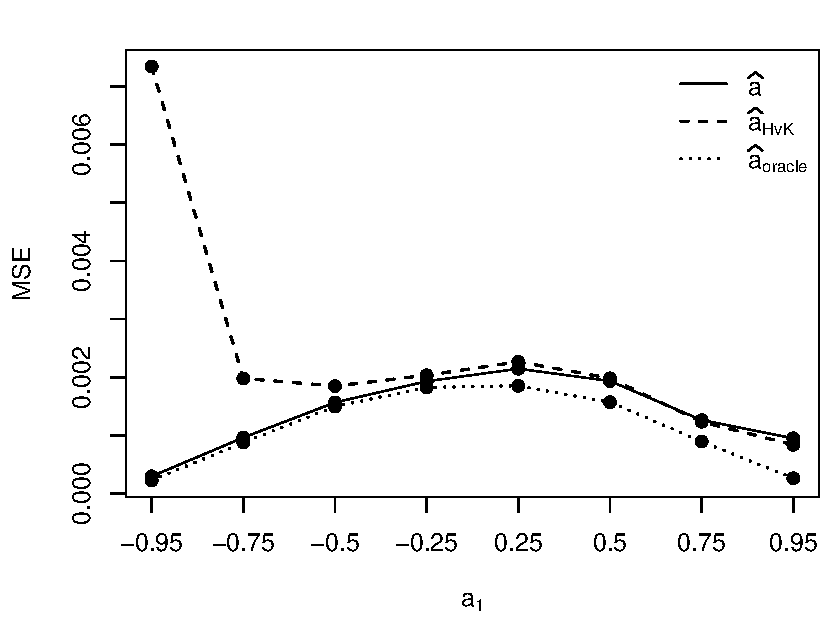
\includegraphics[width=\textwidth]{MSE_a1_T=500_slope=1_(q,r,M1,M2)=(25,10,20,30).pdf}
\end{subfigure}\hspace{0.25cm}
\begin{subfigure}[b]{0.475\textwidth}
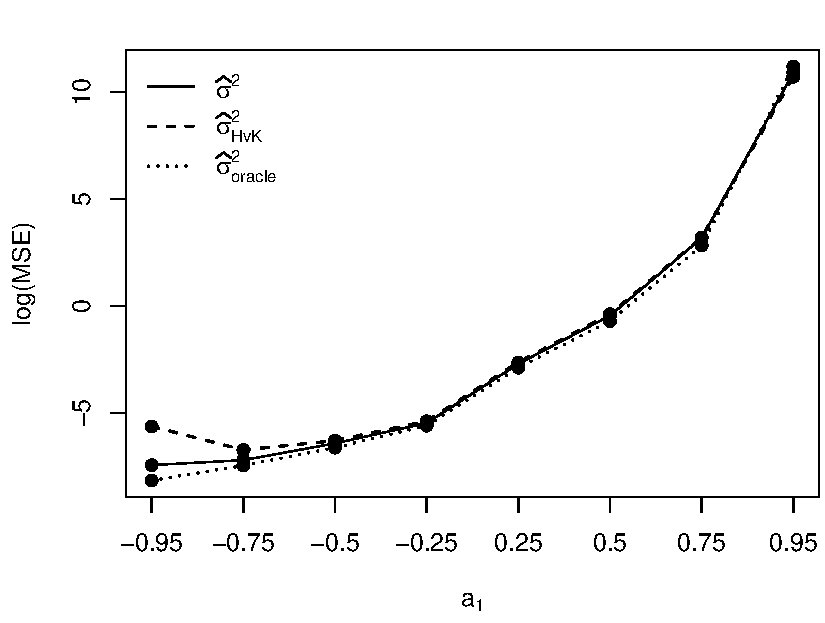
\includegraphics[width=\textwidth]{MSE_lrv_T=500_slope=1_(q,r,M1,M2)=(25,10,20,30).pdf}
\end{subfigure}
\caption{MSE values for the estimators $\widehat{a}$, $\widehat{a}_{\text{HvK}}$, $\widehat{a}_{\text{oracle}}$ and $\widehat{\sigma}^2$, $\widehat{\sigma}^2_{\text{HvK}}$, $\widehat{\sigma}^2_{\text{oracle}}$ in the simulation scenarios for AR($1$) with a moderate trend. %($s_\beta=1$)
}\label{fig:MSE_slope1}
\end{figure}
\end{frame}

\begin{frame}{Simulations}

\begin{figure}[t!]
\begin{subfigure}[b]{0.475\textwidth}
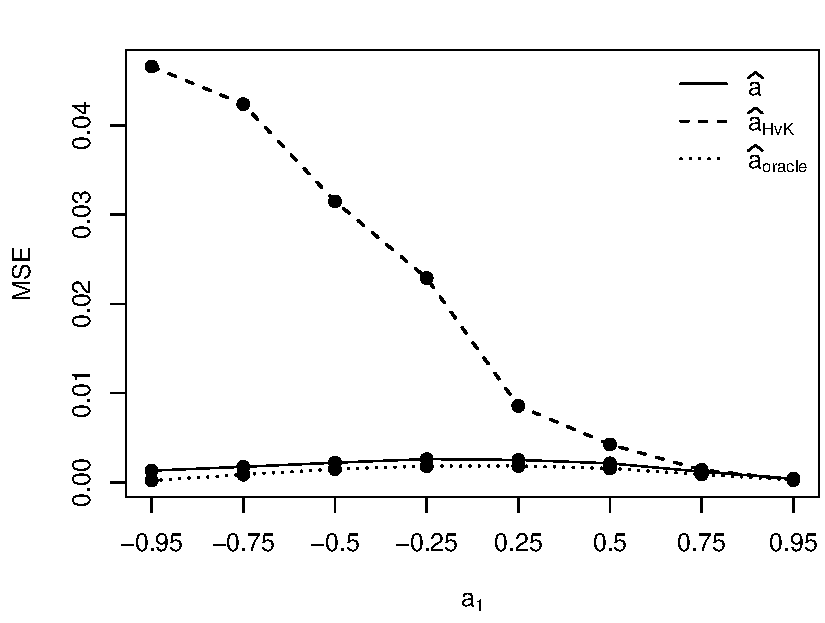
\includegraphics[width=\textwidth]{MSE_a1_T=500_slope=10_(q,r,M1,M2)=(25,10,20,30).pdf}
\end{subfigure}\hspace{0.25cm}
\begin{subfigure}[b]{0.475\textwidth}
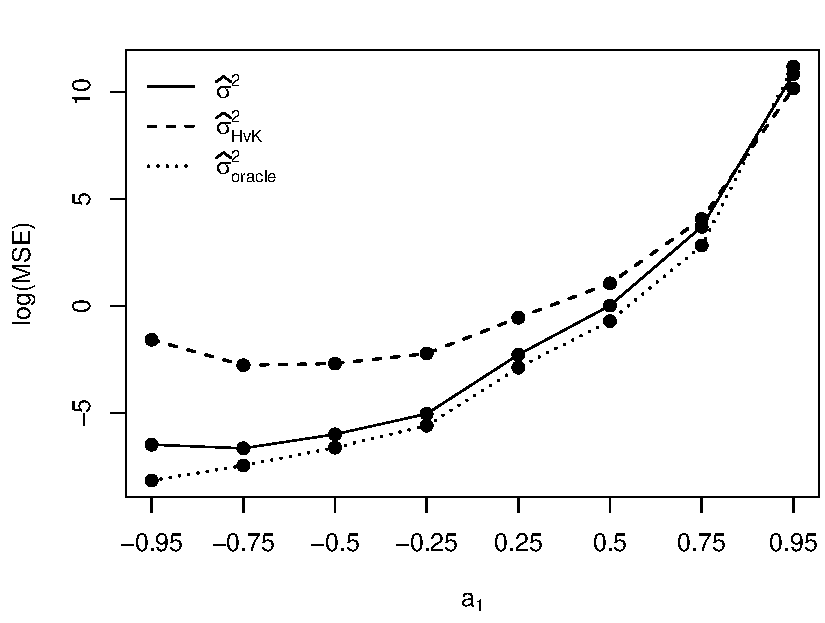
\includegraphics[width=\textwidth]{MSE_lrv_T=500_slope=10_(q,r,M1,M2)=(25,10,20,30).pdf}
\end{subfigure}
\caption{MSE values for the estimators $\widehat{a}$, $\widehat{a}_{\text{HvK}}$, $\widehat{a}_{\text{oracle}}$ and $\widehat{\sigma}^2$, $\widehat{\sigma}^2_{\text{HvK}}$, $\widehat{\sigma}^2_{\text{oracle}}$ in the simulation scenarios for AR($1$) with a pronounced trend.% ($s_\beta=10$).
}\label{fig:MSE_slope10}
\end{figure}
\end{frame}

\begin{frame}{Simulations}


\begin{figure}[t!]
\centering
\begin{subfigure}[b]{0.8\textwidth}
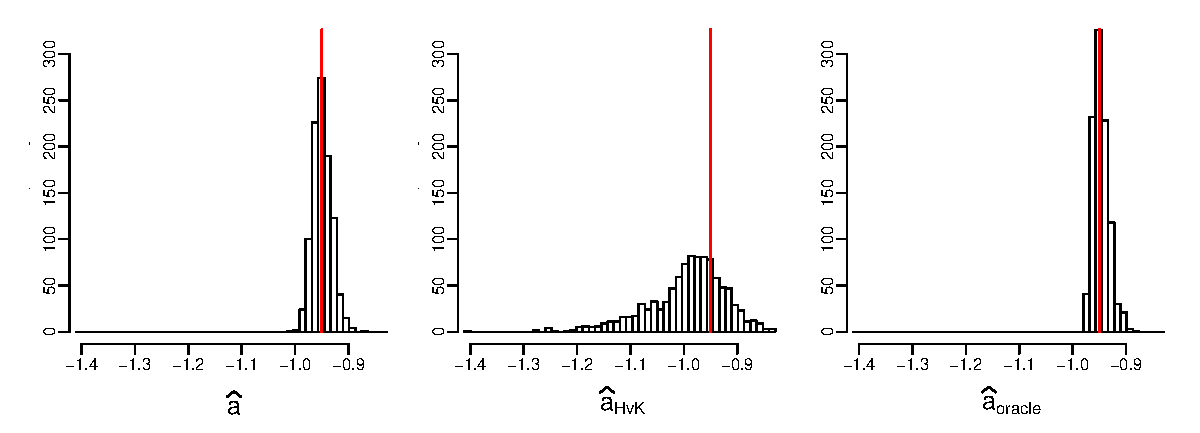
\includegraphics[width=\textwidth]{a_hat_histograms_a1=-95_T=500_slope=1_(q,r,M1,M2)=(25,10,20,30).pdf}
\end{subfigure}
\begin{subfigure}[b]{0.8\textwidth}
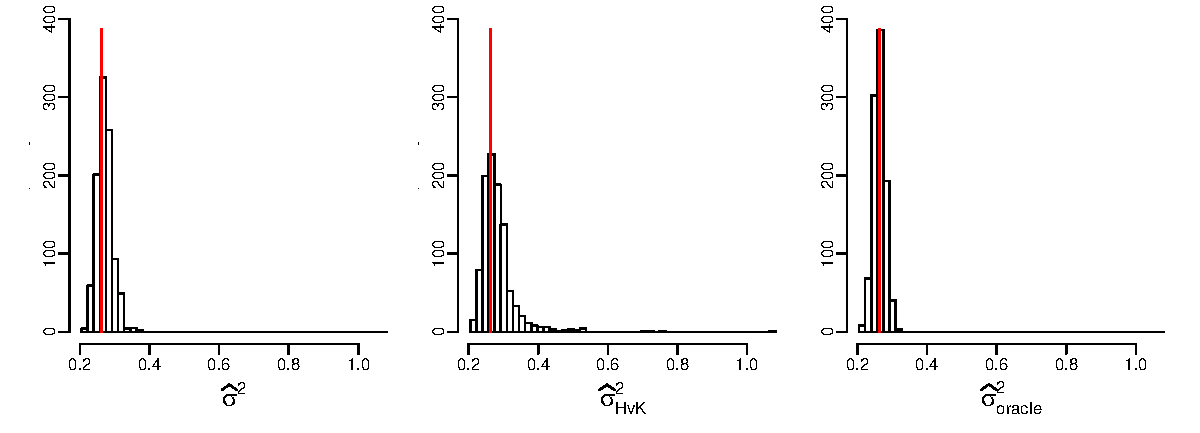
\includegraphics[width=\textwidth]{lrv_histograms_a1=-95_T=500_slope=1_(q,r,M1,M2)=(25,10,20,30).pdf}
\end{subfigure}
\caption{Histograms of the estimators $\widehat{a}$, $\widehat{a}_{\text{HvK}}$, $\widehat{a}_{\text{oracle}}$ and $\widehat{\sigma}^2$, $\widehat{\sigma}^2_{\text{HvK}}$, $\widehat{\sigma}^2_{\text{oracle}}$ in the AR($1$) model with $a_1 = -0.95$ and moderate trend.}\label{fig:hist_scenario1} 
\end{figure}
\end{frame}

\begin{frame}{Simulations}


\begin{figure}[t!]
\centering
\begin{subfigure}[b]{0.8\textwidth}
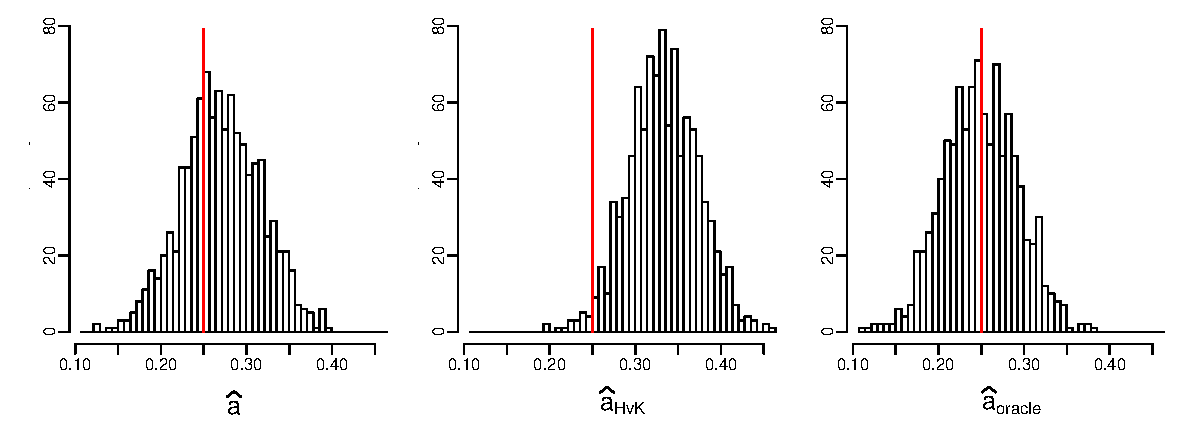
\includegraphics[width=\textwidth]{a_hat_histograms_a1=25_T=500_slope=10_(q,r,M1,M2)=(25,10,20,30).pdf}
\end{subfigure}
\begin{subfigure}[b]{0.8\textwidth}
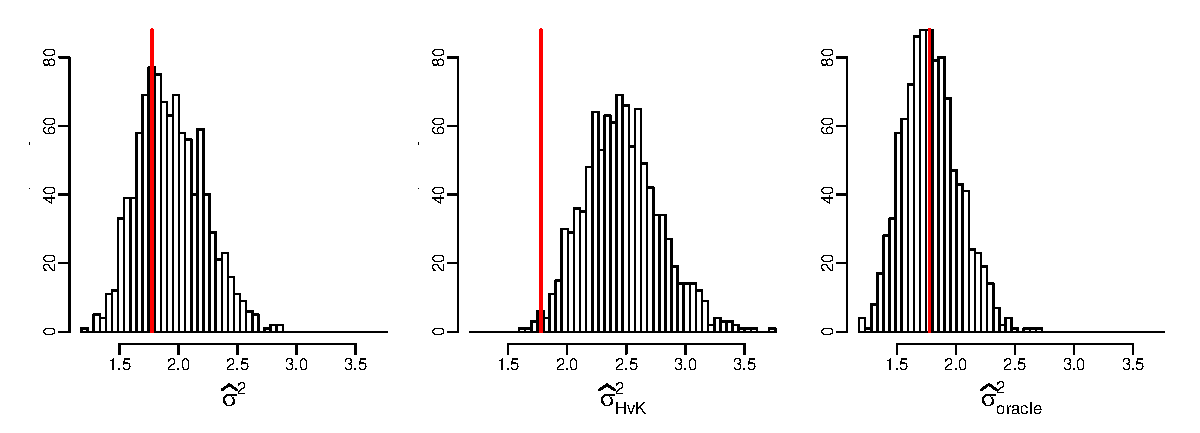
\includegraphics[width=\textwidth]{lrv_histograms_a1=25_T=500_slope=10_(q,r,M1,M2)=(25,10,20,30).pdf}
\end{subfigure}
\caption{Histograms of the estimators $\widehat{a}$, $\widehat{a}_{\text{HvK}}$, $\widehat{a}_{\text{oracle}}$ and $\widehat{\sigma}^2$, $\widehat{\sigma}^2_{\text{HvK}}$, $\widehat{\sigma}^2_{\text{oracle}}$ in the AR($1$) model with $a_1 = 0.25$ and pronounced trend.}\label{fig:hist_scenario2} 
\end{figure}

\end{frame}


\section{Conclusion}
\begin{frame}{Conclusion}
\begin{itemize}
\item We constructed the long-run variance estimator for a wide range of error processes.
\item We proved the $\sqrt{T}$-consistency for our estimators.
\item Our estimator produces accurate estimation results even when the AR polynomial has a root close to the unit circle.
\item In the simulations our estimators tend to perform well even in the presence of a strong trend.
\end{itemize}
\end{frame}

\begin{frame}%[allowframebreaks]
  \frametitle<presentation>{References}    
  \begin{thebibliography}{10}    
  \beamertemplatearticlebibitems
  \bibitem{KhismatullinaVogt2019}
    Khismatullina, M., Vogt, M. (2020)
    \newblock Multiscale inference and long-run variance estimation in nonparametric regression with time series errors.
    \newblock {\em Journal of the Royal Statistical Society: Series B}, 82 5-37.
  %\beamertemplatearticlebibitems
  \bibitem{Hall2003}
  Hall, P. and Van Keilegom, I. (2003).
  \newblock Using difference-based methods for inference in nonparametric regression with time series errors.
    \newblock {\em Journal of the Royal Statistical Society: Series B}, 65 443-456.
  \end{thebibliography}
\end{frame}

\begin{frame}[standout]
  Thank you!
\end{frame}




\appendix


\end{document}
